%%%%%%%%%%%%%%%%%%%%%%%%%%%%%%%%%%%%%%%%%%%%%%%%%%%%%%%%%%%%%%%%%%% 
%                                                                 %
%                            CHAPTER                              %
%                                                                 %
%%%%%%%%%%%%%%%%%%%%%%%%%%%%%%%%%%%%%%%%%%%%%%%%%%%%%%%%%%%%%%%%%%% 

\chapter{Acccelerating the software implementation using HLS}

\section{Analysing software performance}

In the SDSoC environment, it is possible to analyse the software running on the SoC chip using a TCF profiler. After running this analysis, the TCF profiler returns an overview of the functions, sorted on the amount of time spent when running. The analysis is shown in figure \ref{fig:softwareFunctionUsage}

\begin{figure}[H]
	\centering
	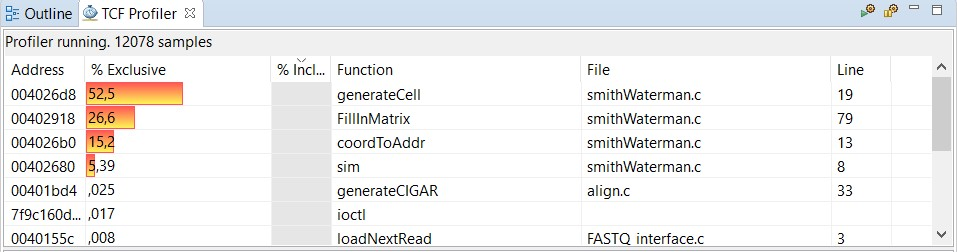
\includegraphics[width=0.75\textwidth]{speedup/softwareFunctionUsage.jpg}
	\caption{a TCF profile of the software implementation}
	\label{fig:softwareFunctionUsage}
\end{figure}

When examining this analysis, we should keep in mind that the generateCell, coordToAddr and sim functions are inline functions used in the FillInMatrix method. Just as suspected the software spends almost all of its time in these methods, so it's worth it to try to accelerate these functions.

\section{Recoding parts of the software to be more hardware friendly}

Back in 2011, Vermij E. did a thesis on RVE (recursive variable expansion). In it, he discusses the most efficient ways to program a processing element to generate one value in the alignment matrix. His results can be found in figure \ref{fig:PE}. 

\begin{figure}[H]
	%src=file:///D:/Erasmus/thesis/interessante%20papers/masterthesis%20Smith-Waterman%20op%20FPGA%20(TU%20Delft).pdf
	\centering
	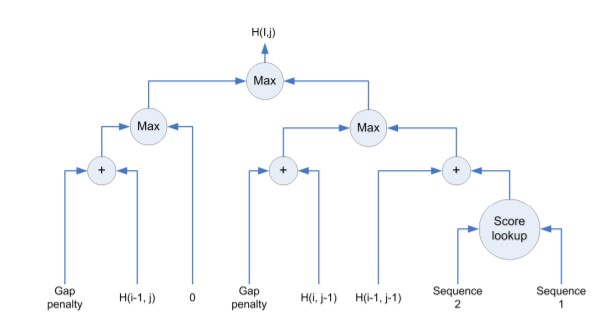
\includegraphics[width=0.75\textwidth]{speedup/PE.jpg}
	\caption{The optimal processing found in the thesis from Vermij E.}
	\label{fig:PE}
\end{figure}

It seemed like a good idea to reimplement the generatecell function, using this newly found scheme. However, it is also important to keep track of where the value comes from. Therefore, the following (new) code was adopted for generating a cell:

\begin{lcverbatim}
//calculate the possible  values
CELL diagonalCELL = { diagonal.value + sim(refVal, seqVal), 1 };
CELL leftCELL = { left.value - gp, 2 };
CELL upCELL = { up.value - gp, 3 };
CELL zeroCELL = { 0, 0 };

CELL upstreamA = (leftCELL.value > upCELL.value) ? leftCELL : upCELL;
CELL upstreamB = (diagonalCELL.value > zeroCELL.value) ? 
					diagonalCELL : zeroCELL;

CELL newCell = (upstreamA.value > upstreamB.value) ? upstreamA : upstreamB;

//Return the cell:
return newCell;
\end{lcverbatim}

Where the second attribute in the CELL type is the direction.

\section{Hardware acceleration}

It turns out, HLS does not support in/out matrix to memory yet.

slices

direction of matrix (first column then row).

Bitwidth of (packed) data on axi master must be power of 2. => change the int to int16\_t and direction to uint16\_t (really wastefull towards memory) but no other choice without major remodel.

\section{Comparison with the software}